\section{实验二:system calls}\label{sec:system calls}

向 xv6 添加一些新的系统调用,理解它们的工作原理,了解 xv6 内核的一些内部原理。

\subsection{实验目的}

\begin{enumerate}
	\item 进一步了解系统调用。
	\item 掌握添加系统调用的方法。
	\item 理解系统调用的工作原理和 xv6 内核的工作过程。
\end{enumerate}

\subsection{实验内容}

\begin{enumerate}
	\item 为 xv6 添加系统调用跟踪功能。
	\item 添加系统调用 \texttt{sysinfo},用于收集正在运行的系统的信息。
\end{enumerate}

\subsection{实验准备}

\begin{enumerate}
	\item 阅读 xv6 参考书的第 2 章,第 4 章的 4.3 和 4.4 节。
	\item 阅读系统调用的用户空间代码 \texttt{user/user.h} 和 \texttt{user/usys.pl}。
	\item 阅读内核空间代码 \texttt{kernel/syscall.h} 和 \texttt{kernel/syscall.c}。
	\item 阅读与进程相关的代码 \texttt{kernel/proc.h} 和 \texttt{kernel/proc.c}。
\end{enumerate}

\subsubsection{机器模式、管理模式、用户模式}

为了实现进程隔离,RISC-V CPU在硬件上提供3种执行命令的模式:机器模式、管理模式(supervisor mode)、用户模式(user mode):

\begin{enumerate}
	\item 机器模式:权限最高,机器模式主要用于配置计算机,配置完成后就会切换到管理模式。
	\item 管理模式:在管理模式下,CPU可以执行privileged instructions(特权指令),比如启用和禁用中断、读取和写入保存页表地址的寄存器等。如果用户模式下的应用程序尝试执行特权指令,则CPU不会执行该指令,而是切换到管理模式。
	\item 用户模式:权限最低,只能执行用户模式指令。要想让CPU从用户模式切换到管理模式,需要调用ecall指令,要想从管理模式切换到用户模式,需要调用sret指令。
\end{enumerate}

\subsubsection{内核组织}

\begin{enumerate}
	\item 单一内核:xv6是一个单一内核。所有系统调用的实现都在内核态的管理模式完成,用户程序通过陷入内核来请求服务。
	\item 微内核:将需要在运行在管理模式下的操作系统代码压缩到最小,保证内核的安全性,将大部分操作系统代码执行放在用户模式。
\end{enumerate}

\begin{figure}[!htb]
	\centering
	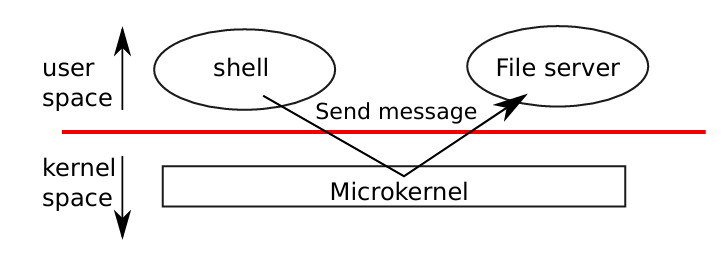
\includegraphics[width=0.75\textwidth]{micro_kernel}
	\caption{带有文件系统的微内核}
	\label{fig:micro_kernel}
\end{figure}

\begin{table}[!hpt]
	\caption{PTE各个位的含义}
	\label{tab:xv6_files}
	\centering
	\begin{tabular}{@{}ll@{}} 		
		\toprule
		\textbf{File} & \textbf{Description} \\
		\midrule
		bio.c         & 文件系统的磁盘块缓存 \\
		console.c     & 用户键盘和屏幕的连接 \\
		entry.S       & 最初的启动指令 \\
		exec.c        & exec() 系统调用 \\
		file.c        & 文件描述符支持 \\
		fs.c          & 文件系统 \\
		kalloc.c      & 物理页分配器 \\
		kernelvec.S   & 处理内核和定时器中断 \\
		log.c         & 文件系统日志与崩溃恢复 \\
		main.c        & 控制引导时其他模块的初始化 \\
		pipe.c        & 管道 \\
		plic.c        & RISC-V中断控制器 \\
		printf.c      & 控制台格式化输出 \\
		proc.c        & 进程与调度 \\
		sleeplock.c   & 会让出CPU的锁 \\
		spinlock.c    & 不会让出CPU的锁 \\
		start.c       & 早期machine模式启动代码 \\
		string.c      & C字符串和字节数组库 \\
		swtch.S       & 线程切换 \\
		syscall.c     & 分发系统调用到处理函数 \\
		sysfile.c     & 文件相关的系统调用 \\
		sysproc.c     & 进程相关的系统调用 \\
		trampoline.S  & 用户与内核切换的汇编代码 \\ 
		trap.c        & 处理中断和trap的C代码 \\
		uart.c        & 串口控制台设备驱动 \\
		virtio\_disk.c & 磁盘设备驱动 \\
		vm.c          & 管理页表和地址空间 \\
		\bottomrule
	\end{tabular}
\end{table}

\subsubsection{进程}

和其他Unix操作系统一样,xv6以进程位隔离单位。每个进程拥有独立的内存空间、CPU执行上下文、文件描述符等资源,防止进程间互相干扰或窃取信息。进程被隔离在用户态,无法直接操作或破坏内核,保证系统安全。

为了实现进程隔离,xv6提供了一种机制让程序认为自己拥有一个独立的机器。一个进程为一个程序提供了一个看似私有的内存系统,或地址空间,其他的进程不能够读/写这个内存。xv6使用page table(页表)来给每个进程分配自己的地址空间,页表再将这些地址空间,也就是进程自己认为的虚拟地址(virtual address)映射到RISC-V实际操作的物理地址(physical address)。

\begin{listing}[!htb]
	\begin{minted}{c}
enum procstate {
    UNUSED, 
    USED, 
    SLEEPING, 
    RUNNABLE, 
    RUNNING, 
    ZOMBIE 
};
	\end{minted}
	\caption{进程的状态定义}\label{lst:procstate}
\end{listing}

\begin{listing}[!htb]
	\begin{minted}{c}
struct proc {
    struct spinlock lock;        // process lock

    // p->lock must be held when using these:
    enum procstate state;        // Process state
    void *chan;                  // If non-zero, sleeping on chan
    int killed;                  // If non-zero, have been killed
    int xstate;                  // Exit status to be returned to parent's wait
    int pid;                     // Process ID

    // wait_lock must be held when using this:
    struct proc *parent;         // Parent process

    // these are private to the process, so p->lock need not be held.
    uint64 kstack;               // Virtual address of kernel stack
    uint64 sz;                   // Size of process memory (bytes)
    pagetable_t pagetable;       // User page table
    struct trapframe *trapframe; // data page for trampoline.S
    struct context context;      // swtch() here to run process
    struct file *ofile[NOFILE];  // Open files
    struct inode *cwd;           // Current directory
    char name[16];               // Process name (debugging)

    int trace_mask;
};
	\end{minted}
	\caption{xv6中进程的定义}\label{lst:proc}
\end{listing}

xv6中进程的详细结构如\cref{lst:proc} 所示。虚拟地址从0开始,往上依次是指令、全局变量、栈、堆。每个进程有两个堆栈:用户堆栈(user stack)和内核堆栈(kernel stack)。当进程在user space中进行时只使用用户堆栈,当进程进入了内核(比如进行了system call)使用内核堆栈。

进程最重要的内核状态有:
\begin{enumerate}
	\item 页表:\texttt{p->pagetable}
	\item 内核堆栈:\texttt{p->kstack}
	\item 运行状态:\texttt{p->state}
\end{enumerate}

\begin{figure}[!htb]
	\centering
	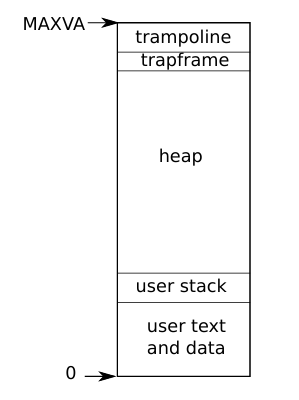
\includegraphics[width=0.45\textwidth]{process_virtual_address}
	\caption{进程虚拟地址空间的布局}
	\label{fig:process_virtual_address}
\end{figure}

\subsubsection{xv6系统调用过程}

xv6系统调用流程图如所示,以下为详细过程:
\begin{enumerate}
	\item 用户空间准备
	
	在user/*.c中,用户程序调用系统调用的接口函数,比如调用 \texttt{write(fd, buf, n)},程序首先调用用户库中定义的接口函数。这个接口函数不是真正的系统调用,而是一个包装函数。
	
	之后。 user/usys.pl 会生成汇编代码 user/usys.S。用户库函数将系统调用的参数依次放入寄存器:第一个参数放入 \texttt{a0},第二个参数放入 \texttt{a1},以此类推,最多支持6个参数。系统调用号则放入 \texttt{a7} 寄存器。
	
	设置完寄存器后,在 user/usys.S 中,用户库函数执行 \texttt{ecall} 指令。这个指令会触发一个异常,使 CPU 从用户模式切换到内核模式,并跳转到内核的异常处理程序。
	
	\item 内核异常处理
	
	\texttt{ecall} 指令执行后,CPU 自动切换到内核模式,并跳转到 kernel/trap.c 的 \texttt{usertrap} 函数。这个函数是内核处理用户空间异常的统一入口点。\texttt{usertrap} 函数首先检查异常的原因。通过读取 \texttt{scause} 寄存器,内核可以判断这是一个系统调用异常是其他类型的异常。如果是系统调用,就调用 \texttt{syscall} 函数;如果是其他异常,则进行相应的处理。
	
	\texttt{syscall} 函数是系统调用的核心分发器。它首先从当前进程的陷阱帧中读取 a7 寄存器的值,这个值就是系统调用号。然后根据系统调用号在系统调用表中查找对应的处理函数。
	 
	\item 参数获取和验证
	
	在 kernel/syscall.c 中,系统调用处理函数(如 sys\_write)需要从用户寄存器中获取参数。内核提供了专门的函数来安全地获取这些参数:	\texttt{argint(n, \&var)} 用于获取第n个整数参数;\texttt{argaddr(n, \&var)} 用于获取第n个地址参数;\texttt{argstr(n, buf, max)} 用于获取第n个字符串参数。这些函数内部都调用 \texttt{argraw(n)} 来从进程的陷阱帧中读取对应的寄存器值。
	
	获取参数后,内核会在文件: kernel/sys*.c (如 kernel/sysproc.c, kernel/sysfile.c)中进行必要的验证,比如检查参数的有效性、验证用户地址是否在进程的地址空间内、检查权限是否足够。
	
	\item 系统调用执行
	
	根据系统调用的类型,内核会调用相应的服务函数。例如:对于文件操作,会调用 kernel/file.c 中的函数;对于进程管理,会调用 kernel/proc.c 中的函数;对于内存管理,会调用 kernel/vm.c 中的函数。这些服务函数执行具体的系统调用逻辑,比如:读取文件内容、创建新进程、分配内存等。
	
	\item 返回结果
	
	如果系统调用需要向用户空间返回数据,内核会使用 kernel/vm.c 中的 \texttt{copyout} 函数将数据从内核空间安全地复制到用户空间,\texttt{copyout} 函数执行的操作包括:验证目标地址的有效性、处理跨页边界的复制、确保复制的安全性。系统调用的返回值通过 \texttt{a0} 寄存器返回给用户程序。成功时通常返回0或正数,失败时返回-1。
	
	\item 返回用户空间
	
	\texttt{usertrap} 函数完成后,会调用 \texttt{usertrapret} 函数来准备返回用户空间。这个函数会恢复用户程序的寄存器状态、设置用户栈指针、准备返回地址。最后执行 \texttt{sret} 指令,CPU 从内核模式切换回用户模式,程序计数器跳转回用户程序中 \texttt{ecall} 指令的下一条指令。用户程序从系统调用返回,获得执行结果,然后继续执行后续的代码。
\end{enumerate}

\begin{figure}[!htb]
	\centering
	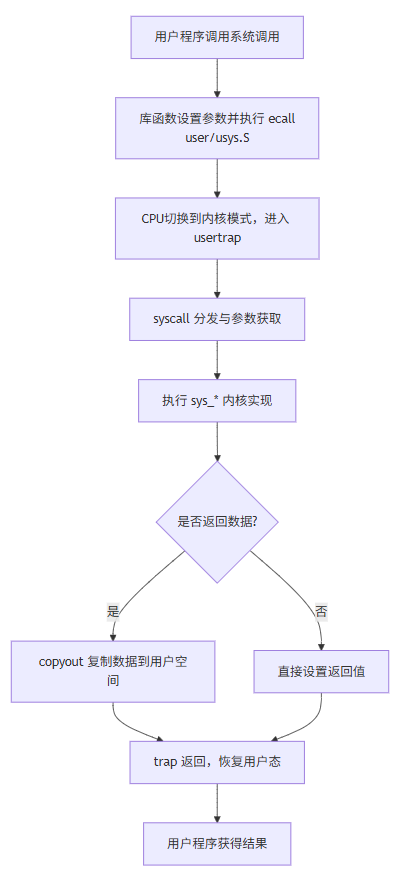
\includegraphics[width=0.5\textwidth]{syscall_steps}
	\caption{xv6系统调用流程图}
	\label{fig:syscall_steps}
\end{figure}

\subsection{实验步骤}

\subsubsection{实现System call tracing}

\begin{enumerate}
	\item 将 \texttt{\$U/\_trace} 添加到 Makefile 中。
	\item 根据题目要求,在 \texttt{kernel/proc.h} 中,为进程结构体 \texttt{proc} 添加成员变量 \texttt{trace\_mask} ,用于表示每一个进程的掩码。如\cref{lst:proc}所示。
	\item 在 \texttt{user/user.h} 中加入代码\texttt{int trace(int)};在\texttt{user/usys.pl}中添加代码\texttt{entry("trace")};在 \texttt{kernel/syscall} 中添加代码 \texttt{\#define SYS\_trace 22};
	\item 在 \texttt{kernel/syscall.c} 中添加一个数组\texttt{static char *syscall\_name[]},用于记录每个进程的名称。如\cref{lst:syscall_name}所示
	\item 修改 \texttt{kernel/syscall.c} 中的 \texttt{syscall} 函数,增加两行,通过掩码和编号做与运算进行输出。如\cref{lst:syscall}所示。
	\item 修改 \texttt{kernel/proc.c} 中的 \texttt{fork} 函数,添加一行 \texttt{np->trace\_mask = p->trace\_mask},传递mask参数。
	\item 在 \texttt{kernel/sysproc.c} 中添加一个 \texttt{sys\_trace()} 函数,将参数传递给 \texttt{trace\_mask} 即可。如\cref{lst:sys_trace}所示。
	\item 测试 trace 方法,成功运行。如\cref{fig:test_trace(1)}和\cref{fig:test_trace(2)}所示。
\end{enumerate}

\begin{listing}[!htb]
	\begin{minted}{c}
static char *syscall_name[] = {
    "fork",    // SYS_fork
    "exit",    // SYS_exit
    "wait",    // SYS_wait
    "pipe",    // SYS_pipe
    "read",    // SYS_read
    "kill",    // SYS_kill
    "exec",    // SYS_exec
    "fstat",   // SYS_fstat
    "chdir",   // SYS_chdir
    "dup",     // SYS_dup
    "getpid",  // SYS_getpid
    "sbrk",    // SYS_sbrk
    "sleep",   // SYS_sleep
    "uptime",  // SYS_uptime
    "open",    // SYS_open
    "write",   // SYS_write
    "mknod",   // SYS_mknod
    "unlink",  // SYS_unlink
    "link",    // SYS_link
    "mkdir",   // SYS_mkdir
    "close",   // SYS_close
    "trace",   // SYS_trace
    "sysinfo"  // SYS_sysinfo
};
	\end{minted}
	\caption{记录进程名称的数组}\label{lst:syscall_name}
\end{listing}

\begin{listing}[!htb]
	\begin{minted}{c}
void
syscall(void)
{
    int num;
    struct proc *p = myproc();
    
    num = p->trapframe->a7;
    if(num > 0 && num < NELEM(syscalls) && syscalls[num]) {
        p->trapframe->a0 = syscalls[num]();
        if((p->trace_mask>>num)&1){
            printf("%d: syscall %s -> %d\n",p->pid,syscall_name[num-1],p->trapframe->a0);
        }
    } else {
        printf("%d %s: unknown sys call %d\n",
        p->pid, p->name, num);
        p->trapframe->a0 = -1;
    }
}
	\end{minted}
	\caption{syscall函数的实现}\label{lst:syscall}
\end{listing}

\begin{listing}[!htb]
	\begin{minted}{c}
uint64
sys_trace(void)
{
    int mask;
    if(argint(0, &mask) < 0){
        return -1;
    }

    struct proc *p = myproc();
    p->trace_mask = mask;
    return 0;
}
	\end{minted}
	\caption{sys\_trace函数的实现}\label{lst:sys_trace}
\end{listing}

\begin{figure}[!htb]
	\centering
	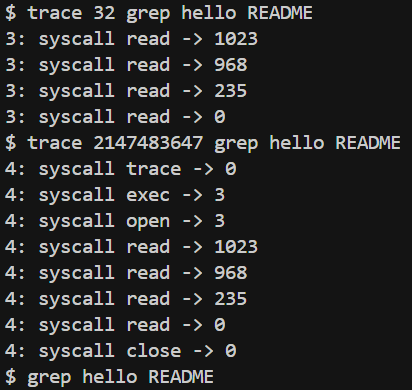
\includegraphics[width=0.4\textwidth]{test_trace(1)}
	\caption{测试trace方法(1)}
	\label{fig:test_trace(1)}
\end{figure}

\begin{figure}[!htb]
	\centering
	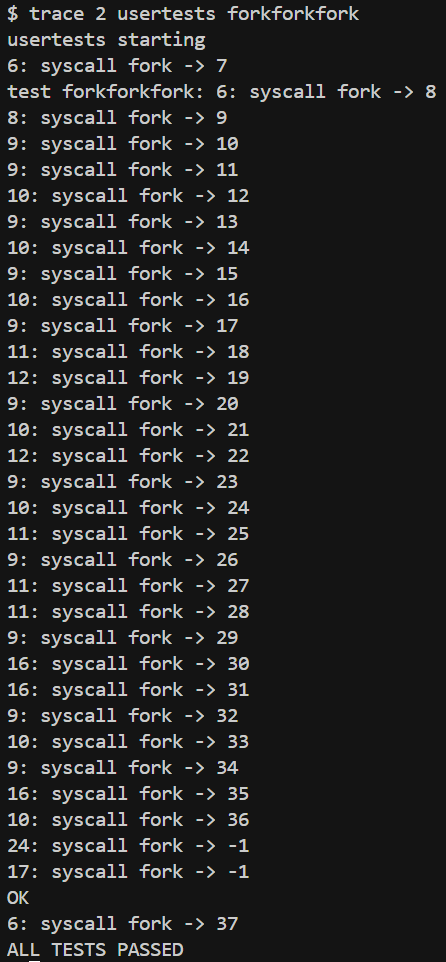
\includegraphics[width=0.4\textwidth]{test_trace(2)}
	\caption{测试trace方法(2)}
	\label{fig:test_trace(2)}
\end{figure}

\subsubsection{实现Sysinfo}

统计可用的内存数量:

\begin{enumerate}
	\item 根据提示,阅读代码 \texttt{kernel/kalloc.c}。
	\item 在 \texttt{kalloc.c} 中,\cref{lst:kmem}包含了空闲地址的链表指针。
	\item 要统计可用的内存空间大小,需要遍历空闲链表 \texttt{freelist},统计链表节点个数,在乘以单个内存页的大小 \texttt{PGSIZE}。
	\item 参考文件中的其他函数,实现统计功能\texttt{collect\_used\_proc},如\cref{lst:collect_freemem}所示。
	\item 需要注意,在进行统计操作时需要上锁。
\end{enumerate}

\begin{listing}[!htb]
	\begin{minted}{c}
struct {
	struct spinlock lock;    // Spinlock to protect the free list.
	struct run *freelist;    // Pointer to the head of the free list.
} kmem;
	\end{minted}
	\caption{物理内存分配器定义}\label{lst:kmem}
\end{listing}

\begin{listing}[!htb]
	\begin{minted}{c}
int collect_freemem(){
    struct run *r;
    int free_memory_count = 0;
    acquire(&kmem.lock);
    r = kmem.freelist;
    while(r){
        r = r->next;
        free_memory_count++;
    }
    release(&kmem.lock);
    return free_memory_count * PGSIZE;
}
	\end{minted}
	\caption{统计可用的内存空间大小}\label{lst:collect_freemem}
\end{listing}

统计已使用的进程数量:

\begin{enumerate}
	\item 根据提示,阅读代码 \texttt{kernel/proc.c} 和 \texttt{kernel/proc.h};
	\item 在 \texttt{proc.c}中,\cref{lst:proc-array}保存着所有的进程,进程的状态存储在,\cref{lst:procstate}中。
	\item 要统计未使用进程的数量,即为统计 \texttt{PCB} 表 \texttt{proc} 中进程状态不是 \texttt{UNUESD} 的进程数量。
	\item 参考文件中的其他函数,实现统计功能 \texttt{collect\_used\_proc} ,如\cref{lst:collect_used_proc}所示。
	\item 需要注意,在进行统计操作时需要上锁。
\end{enumerate}

\begin{listing}[!htb]
	\begin{minted}{c}
struct proc proc[NPROC]; 
	\end{minted}
	\caption{PCB表的定义}\label{lst:proc_array}
\end{listing}

\begin{listing}[!htb]
	\begin{minted}{c}
int
collect_used_proc(){
    struct proc *p;
    int used_proc_cnt = 0;

    for(p = proc;p < &proc[NPROC];p++){
        acquire(&p->lock);
        if(p->state != UNUSED){
            used_proc_cnt++;
        }
        release(&p->lock);
    }
    return used_proc_cnt;
}
	\end{minted}
	\caption{collect\_used\_proc函数的实现}\label{lst:collect_used_proc}
\end{listing}

Sysinfo实现:
\begin{enumerate}
	\item 将 \texttt{\$U/\_sysinfotest} 添加到 Makefile 中。
	\item 在 \texttt{user/user.h} 中声明结构体 \texttt{sysinfo} 并加入代码 \texttt{int sysinfo(struct sysinfo *)};在 \texttt{user/usys.pl} 中添加代码 \texttt{entry("sysinfo")};在 \texttt{kernel/syscall} 中添加代码 \texttt{\#define SYS\_sysinfo 23};
	\item 在 \texttt{kernel/defs.h} 中,声明函数 \texttt{collect\_freemem} 和 \texttt{collect\_used\_proc}。
	\item 在 \texttt{kernel/sysproc.c} 中,创建函数 \texttt{sys\_sysinfo},通过 \texttt{argaddr} 传递地址参数,将可用内存大小和已使用进程数量赋值给 \texttt{sysinfo} 收集有关正在运行的系统的信息,如\cref{lst:sys_sysinfo}所示。
	\item 测试 sysinfo 方法,成功运行。如\cref{fig:test_sysinfo} 所示。
\end{enumerate}

\begin{figure}[!htb]
	\centering
	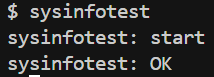
\includegraphics[width=0.4\textwidth]{test_sysinfo}
	\caption{测试sysinfo方法}
	\label{fig:test_sysinfo}
\end{figure}

\begin{listing}[!htb]
	\begin{minted}{c}
uint64
sys_sysinfo(void)
{
    struct sysinfo info;
    uint64 addr;
    struct proc *p = myproc();

    info.nproc = collect_used_proc();
    info.freemem = collect_freemem();
    if(argaddr(0, &addr) < 0)
        return -1;
    
    if(copyout(p->pagetable, addr, (char *)&info, sizeof(info)) < 0)
        return -1; 
    return 0;
}
	\end{minted}
	\caption{sys\_sysinfo函数的实现}\label{lst:sys_sysinfo}
\end{listing}

\subsubsection{综合测试}

在xv6-labs-2021目录下创建一个time.txt文件,记录我完成该lab花费的时间,使用\texttt{make grade}对lab1进行综合测试,测试通过。

\begin{figure}[!htb]
	\centering
	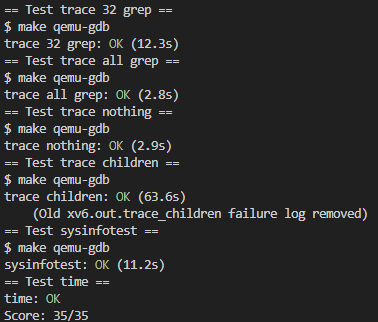
\includegraphics[width=0.5\textwidth]{test_lab2}
	\caption{lab2综合测试}
	\label{fig:test_lab2}
\end{figure}

\subsection{实验小结}

本次实验实际上是对系统调用的深入理解,在做这次实验的过程中我遇到的问题相对比较多。在第一个 trace 的过程中,需要阅读比较多的内核 kernel 源代码,包括 syscall()等函数,只有熟悉了这些函数才能够比较好的完成实验内容。

在完成第二部分 sysinfo 的时候,由于对进程的定义仅仅停留在课本上,因此刚开始的时候难以下手。但是通过查阅相关资料,我了解到 xv6 中存储所有进程的变量和进程状态变量,仿照着已经存在的内核函数,终于完成了该部分。

不过,尽管完成了该实验,但是我还是存在一些疑惑,比如 user/user.h 和 kernel/syscall.h 究竟是如何起作用的?在一众C语言中,为什么user/usys.pl采用perl语言,它又是如何起作用的?希望这些疑惑能我能在接下来的学习中得到解答。

总体来说,这次实验让我在实验一的基础上更加了解系统调用,同时也为未来的实验打下了比较扎实的基础。此外,也让我更加熟悉了写系统调用的方法, 对内核和用户也有了比较好的区分。
